%This file will discuss solutions implemented
%This file should be included in doc using \input{file}

\section{Proposed Solutions}

\subsection{Simulations}

\subsection{Physical Implementation}

The proposed solution incorporates the following components for the physical system architecture.

\begin{itemize}
\item Joystick Controller
\item Base Station Laptop
\item Raspberry Pi 3 Computer
\item Arduino Micro-Controller
\item 10 Degree of Freedom Inertial Measurement Unit
\item Raspberry Pi Camera Module (Future)
\end{itemize}

The system architecture is implemented as depicted in the block diagram shown in Figure \ref{fig:sys_arch}. 

\begin{figure}[H]
	\centering
	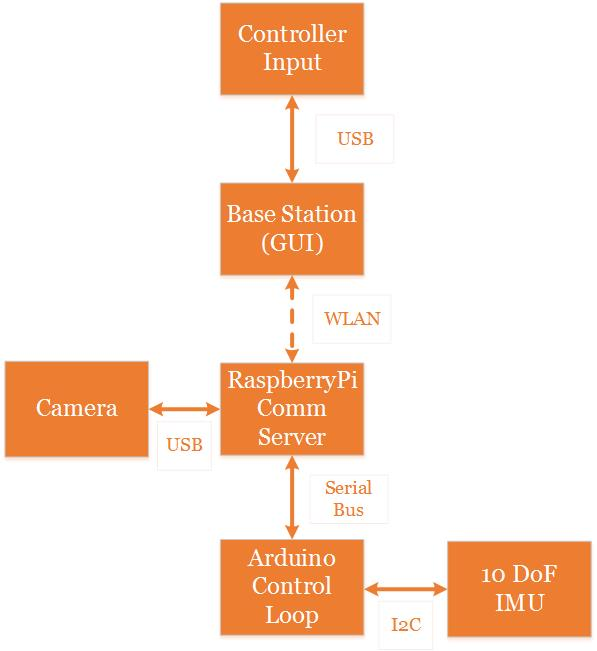
\includegraphics[width=0.7\textwidth]{flowchart-architecture.jpg}
	\caption{System Architecture}
	\label{fig:sys_arch}	
\end{figure}

A joystick controller was used as the control input for its non-spring loaded throttle control. The drone requires an altitude set point from the control input, a spring loaded control input would make the implementation of a constant set point difficult. The base station laptop hosts the GUI and the communication channel software between the USB connected joystick control input and the Raspberry Pi Wi-Fi connection. The Python scripts that enable the communication channels use the sockets library for a server, client Wi-Fi channel and pygame library to acquire control set points from the joystick controller. 


\subsection{Graphical User Interface}
\subsubsection{Framework Selection}
The basic GUI was to have the ability to call the PS4 controller initialization script and manipulate the axis settings. Because the initialization script was written in Python it was very difficult and time consuming to do this using the C++ version of Qt compared to using PyQt5 where all that had to be done was import the script. Because each of the scripts that the GUI needs to call are written using Python it was decided to carry on using PyQt5. On top of the ease of importing the scripts using PyQt5 it also allows us to use the vast amount of Python libraries that are available.

